\documentclass[twoside]{book}

% Packages required by doxygen
\usepackage{fixltx2e}
\usepackage{calc}
\usepackage{doxygen}
\usepackage[export]{adjustbox} % also loads graphicx
\usepackage{graphicx}
\usepackage[utf8]{inputenc}
\usepackage{makeidx}
\usepackage{multicol}
\usepackage{multirow}
\PassOptionsToPackage{warn}{textcomp}
\usepackage{textcomp}
\usepackage[nointegrals]{wasysym}
\usepackage[table]{xcolor}

% Font selection
\usepackage[T1]{fontenc}
\usepackage[scaled=.90]{helvet}
\usepackage{courier}
\usepackage{amssymb}
\usepackage{sectsty}
\renewcommand{\familydefault}{\sfdefault}
\allsectionsfont{%
  \fontseries{bc}\selectfont%
  \color{darkgray}%
}
\renewcommand{\DoxyLabelFont}{%
  \fontseries{bc}\selectfont%
  \color{darkgray}%
}
\newcommand{\+}{\discretionary{\mbox{\scriptsize$\hookleftarrow$}}{}{}}

% Page & text layout
\usepackage{geometry}
\geometry{%
  a4paper,%
  top=2.5cm,%
  bottom=2.5cm,%
  left=2.5cm,%
  right=2.5cm%
}
\tolerance=750
\hfuzz=15pt
\hbadness=750
\setlength{\emergencystretch}{15pt}
\setlength{\parindent}{0cm}
\setlength{\parskip}{3ex plus 2ex minus 2ex}
\makeatletter
\renewcommand{\paragraph}{%
  \@startsection{paragraph}{4}{0ex}{-1.0ex}{1.0ex}{%
    \normalfont\normalsize\bfseries\SS@parafont%
  }%
}
\renewcommand{\subparagraph}{%
  \@startsection{subparagraph}{5}{0ex}{-1.0ex}{1.0ex}{%
    \normalfont\normalsize\bfseries\SS@subparafont%
  }%
}
\makeatother

% Headers & footers
\usepackage{fancyhdr}
\pagestyle{fancyplain}
\fancyhead[LE]{\fancyplain{}{\bfseries\thepage}}
\fancyhead[CE]{\fancyplain{}{}}
\fancyhead[RE]{\fancyplain{}{\bfseries\leftmark}}
\fancyhead[LO]{\fancyplain{}{\bfseries\rightmark}}
\fancyhead[CO]{\fancyplain{}{}}
\fancyhead[RO]{\fancyplain{}{\bfseries\thepage}}
\fancyfoot[LE]{\fancyplain{}{}}
\fancyfoot[CE]{\fancyplain{}{}}
\fancyfoot[RE]{\fancyplain{}{\bfseries\scriptsize Generated by Doxygen }}
\fancyfoot[LO]{\fancyplain{}{\bfseries\scriptsize Generated by Doxygen }}
\fancyfoot[CO]{\fancyplain{}{}}
\fancyfoot[RO]{\fancyplain{}{}}
\renewcommand{\footrulewidth}{0.4pt}
\renewcommand{\chaptermark}[1]{%
  \markboth{#1}{}%
}
\renewcommand{\sectionmark}[1]{%
  \markright{\thesection\ #1}%
}

% Indices & bibliography
\usepackage{natbib}
\usepackage[titles]{tocloft}
\setcounter{tocdepth}{3}
\setcounter{secnumdepth}{5}
\makeindex

% Hyperlinks (required, but should be loaded last)
\usepackage{ifpdf}
\ifpdf
  \usepackage[pdftex,pagebackref=true]{hyperref}
\else
  \usepackage[ps2pdf,pagebackref=true]{hyperref}
\fi
\hypersetup{%
  colorlinks=true,%
  linkcolor=blue,%
  citecolor=blue,%
  unicode%
}

% Custom commands
\newcommand{\clearemptydoublepage}{%
  \newpage{\pagestyle{empty}\cleardoublepage}%
}

\usepackage{caption}
\captionsetup{labelsep=space,justification=centering,font={bf},singlelinecheck=off,skip=4pt,position=top}

%===== C O N T E N T S =====

\begin{document}

% Titlepage & ToC
\hypersetup{pageanchor=false,
             bookmarksnumbered=true,
             pdfencoding=unicode
            }
\pagenumbering{alph}
\begin{titlepage}
\vspace*{7cm}
\begin{center}%
{\Large My Project }\\
\vspace*{1cm}
{\large Generated by Doxygen 1.8.14}\\
\end{center}
\end{titlepage}
\clearemptydoublepage
\pagenumbering{roman}
\tableofcontents
\clearemptydoublepage
\pagenumbering{arabic}
\hypersetup{pageanchor=true}

%--- Begin generated contents ---
\chapter{Modèle de conception Observateur}
\label{index}\hypertarget{index}{}L\textquotesingle{}implémentation du {\itshape desing pattern} \href{https://en.wikipedia.org/wiki/Observer_pattern}{\tt Observer} donnée ici est fidèle au modèle du \href{https://en.wikipedia.org/wiki/Design_Patterns}{\tt Gang of Four}. En particulier, il n\textquotesingle{}y est pas fait usage d\textquotesingle{}une classe correspondant aux {\itshape événements}, mais uniquement d\textquotesingle{}une classe {\itshape source d\textquotesingle{}événements}, le sujet \mbox{\hyperlink{classnvs_1_1_subject}{nvs\+::\+Subject}}, et d\textquotesingle{}une classe {\itshape écouteur d\textquotesingle{}événements}, l\textquotesingle{}observateur \mbox{\hyperlink{classnvs_1_1_observer}{nvs\+::\+Observer}}.

Dans ses mises en œuvre effective, ce modèle est très souvent étoffé par l\textquotesingle{}ajout de classes d\textquotesingle{}événement ou par la multiplication des méthodes de notification. Rien, cependant, de ce que ces complexifications du modèle rendent plus facile aux utilisateurs, n\textquotesingle{}est hors de portée du modèle simple donné ici. Les développements du modèle de conception peuvent en effet être reportées sur les classes concrètes qui l\textquotesingle{}implémentent. Remarquez que si le contenu de ce paragraphe vous semble abscons, oubliez-\/le provisoirement. On en reparle lors de la \href{https://doc.qt.io/qt-5/eventsandfilters.html}{\tt gestion des événements avec Qt}. 
\chapter{Namespace Index}
\section{Namespace List}
Here is a list of all documented namespaces with brief descriptions\+:\begin{DoxyCompactList}
\item\contentsline{section}{\mbox{\hyperlink{namespacenvs}{nvs}} \\*Espace de nom de Nicolas Vansteenkiste }{\pageref{namespacenvs}}{}
\end{DoxyCompactList}

\chapter{Hierarchical Index}
\section{Class Hierarchy}
This inheritance list is sorted roughly, but not completely, alphabetically\+:\begin{DoxyCompactList}
\item \contentsline{section}{nvs\+:\+:Observer}{\pageref{classnvs_1_1_observer}}{}
\begin{DoxyCompactList}
\item \contentsline{section}{Window}{\pageref{class_window}}{}
\end{DoxyCompactList}
\item Q\+Grid\+Layout\begin{DoxyCompactList}
\item \contentsline{section}{Board}{\pageref{class_board}}{}
\item \contentsline{section}{Box}{\pageref{class_box}}{}
\end{DoxyCompactList}
\item Q\+Widget\begin{DoxyCompactList}
\item \contentsline{section}{Window}{\pageref{class_window}}{}
\end{DoxyCompactList}
\item \contentsline{section}{nvs\+:\+:Subject}{\pageref{classnvs_1_1_subject}}{}
\end{DoxyCompactList}

\chapter{Class Index}
\section{Class List}
Here are the classes, structs, unions and interfaces with brief descriptions\+:\begin{DoxyCompactList}
\item\contentsline{section}{\mbox{\hyperlink{class_board}{Board}} }{\pageref{class_board}}{}
\item\contentsline{section}{\mbox{\hyperlink{class_box}{Box}} }{\pageref{class_box}}{}
\item\contentsline{section}{\mbox{\hyperlink{classnvs_1_1_observer}{nvs\+::\+Observer}} \\*Classe abstraite de base de tout observateur }{\pageref{classnvs_1_1_observer}}{}
\item\contentsline{section}{\mbox{\hyperlink{classnvs_1_1_subject}{nvs\+::\+Subject}} \\*Classe de base de tout \char`\"{}sujet d\textquotesingle{}observation\char`\"{} }{\pageref{classnvs_1_1_subject}}{}
\item\contentsline{section}{\mbox{\hyperlink{class_window}{Window}} }{\pageref{class_window}}{}
\end{DoxyCompactList}

\chapter{File Index}
\section{File List}
Here is a list of all documented files with brief descriptions\+:\begin{DoxyCompactList}
\item\contentsline{section}{C\+:/\+Users/benaz/\+Documents/cpp+/\+Labyrinth\+Project/{\bfseries board.\+h} }{\pageref{board_8h}}{}
\item\contentsline{section}{C\+:/\+Users/benaz/\+Documents/cpp+/\+Labyrinth\+Project/{\bfseries box.\+h} }{\pageref{box_8h}}{}
\item\contentsline{section}{C\+:/\+Users/benaz/\+Documents/cpp+/\+Labyrinth\+Project/\mbox{\hyperlink{observer_8h}{observer.\+h}} \\*Définition de la classe \mbox{\hyperlink{classnvs_1_1_observer}{nvs\+::\+Observer}} }{\pageref{observer_8h}}{}
\item\contentsline{section}{C\+:/\+Users/benaz/\+Documents/cpp+/\+Labyrinth\+Project/\mbox{\hyperlink{subject_8cpp}{subject.\+cpp}} \\*Implémentation de la classe \mbox{\hyperlink{classnvs_1_1_subject}{nvs\+::\+Subject}} }{\pageref{subject_8cpp}}{}
\item\contentsline{section}{C\+:/\+Users/benaz/\+Documents/cpp+/\+Labyrinth\+Project/\mbox{\hyperlink{subject_8h}{subject.\+h}} \\*Définition de la classe \mbox{\hyperlink{classnvs_1_1_subject}{nvs\+::\+Subject}} }{\pageref{subject_8h}}{}
\item\contentsline{section}{C\+:/\+Users/benaz/\+Documents/cpp+/\+Labyrinth\+Project/{\bfseries window.\+h} }{\pageref{window_8h}}{}
\end{DoxyCompactList}

\chapter{Namespace Documentation}
\hypertarget{namespacenvs}{}\section{nvs Namespace Reference}
\label{namespacenvs}\index{nvs@{nvs}}


Espace de nom de Nicolas Vansteenkiste.  


\subsection*{Classes}
\begin{DoxyCompactItemize}
\item 
class \mbox{\hyperlink{classnvs_1_1_observer}{Observer}}
\begin{DoxyCompactList}\small\item\em Classe abstraite de base de tout observateur. \end{DoxyCompactList}\item 
class \mbox{\hyperlink{classnvs_1_1_subject}{Subject}}
\begin{DoxyCompactList}\small\item\em Classe de base de tout \char`\"{}sujet d\textquotesingle{}observation\char`\"{}. \end{DoxyCompactList}\end{DoxyCompactItemize}


\subsection{Detailed Description}
Espace de nom de Nicolas Vansteenkiste. 
\chapter{Class Documentation}
\hypertarget{class_board}{}\section{Board Class Reference}
\label{class_board}\index{Board@{Board}}
Inheritance diagram for Board\+:\begin{figure}[H]
\begin{center}
\leavevmode
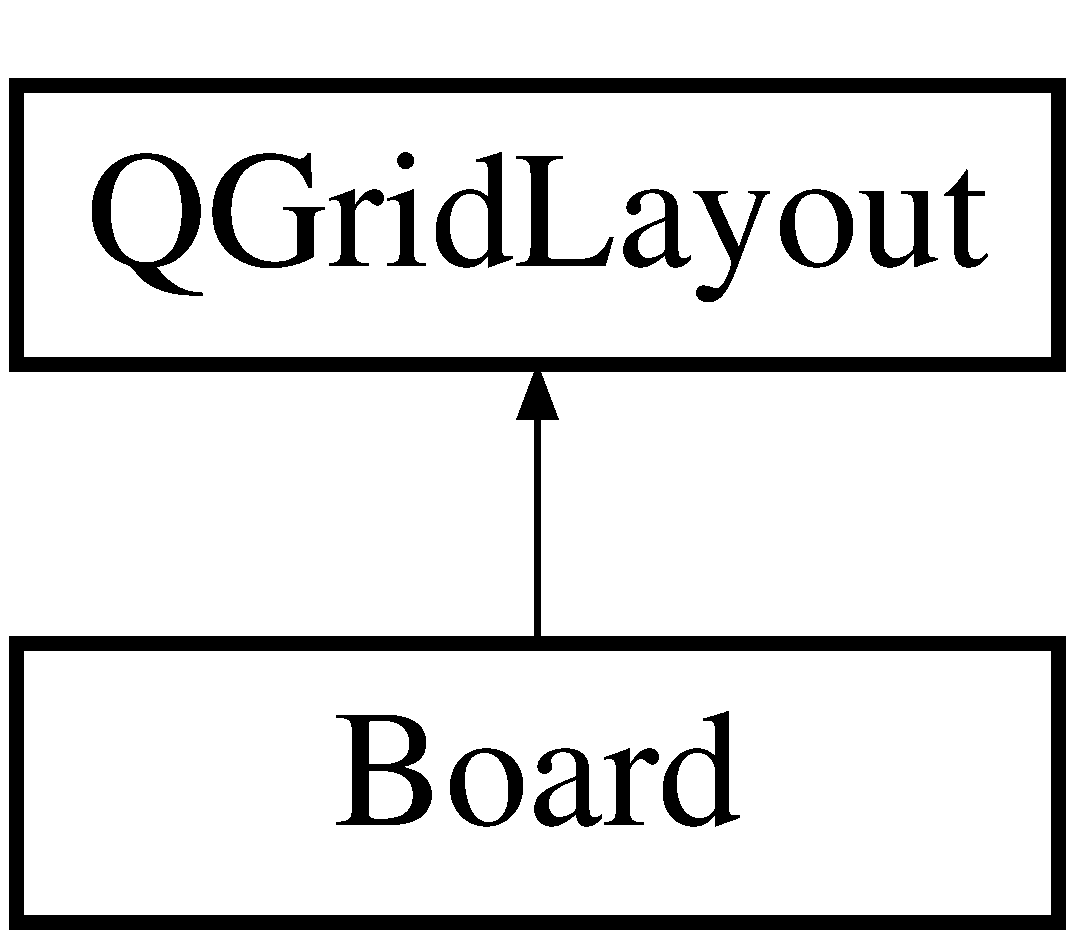
\includegraphics[height=2.000000cm]{class_board}
\end{center}
\end{figure}
\subsection*{Public Member Functions}
\begin{DoxyCompactItemize}
\item 
\mbox{\hyperlink{class_board_ac3267e47810e8951899b852daa9d2f38}{Board}} (Labyrinth $\ast$game)
\begin{DoxyCompactList}\small\item\em constructeur \mbox{\hyperlink{class_board}{Board}} \end{DoxyCompactList}\item 
\mbox{\Hypertarget{class_board_aa170cb05bb38de48e19a72b51d898eca}\label{class_board_aa170cb05bb38de48e19a72b51d898eca}} 
void \mbox{\hyperlink{class_board_aa170cb05bb38de48e19a72b51d898eca}{update}} ()
\begin{DoxyCompactList}\small\item\em update mets a jour le board. \end{DoxyCompactList}\end{DoxyCompactItemize}
\subsection*{Private Attributes}
\begin{DoxyCompactItemize}
\item 
\mbox{\Hypertarget{class_board_afc223806fde02c0bda335aa365d82b4d}\label{class_board_afc223806fde02c0bda335aa365d82b4d}} 
Labyrinth $\ast$ {\bfseries game\+\_\+}
\end{DoxyCompactItemize}


\subsection{Constructor \& Destructor Documentation}
\mbox{\Hypertarget{class_board_ac3267e47810e8951899b852daa9d2f38}\label{class_board_ac3267e47810e8951899b852daa9d2f38}} 
\index{Board@{Board}!Board@{Board}}
\index{Board@{Board}!Board@{Board}}
\subsubsection{\texorpdfstring{Board()}{Board()}}
{\footnotesize\ttfamily Board\+::\+Board (\begin{DoxyParamCaption}\item[{Labyrinth $\ast$}]{game }\end{DoxyParamCaption})}



constructeur \mbox{\hyperlink{class_board}{Board}} 


\begin{DoxyParams}{Parameters}
{\em game} & \\
\hline
\end{DoxyParams}


The documentation for this class was generated from the following files\+:\begin{DoxyCompactItemize}
\item 
C\+:/\+Users/benaz/\+Documents/cpp+/\+Labyrinth\+Project/board.\+h\item 
C\+:/\+Users/benaz/\+Documents/cpp+/\+Labyrinth\+Project/board.\+cpp\end{DoxyCompactItemize}

\hypertarget{class_box}{}\section{Box Class Reference}
\label{class_box}\index{Box@{Box}}
Inheritance diagram for Box\+:\begin{figure}[H]
\begin{center}
\leavevmode
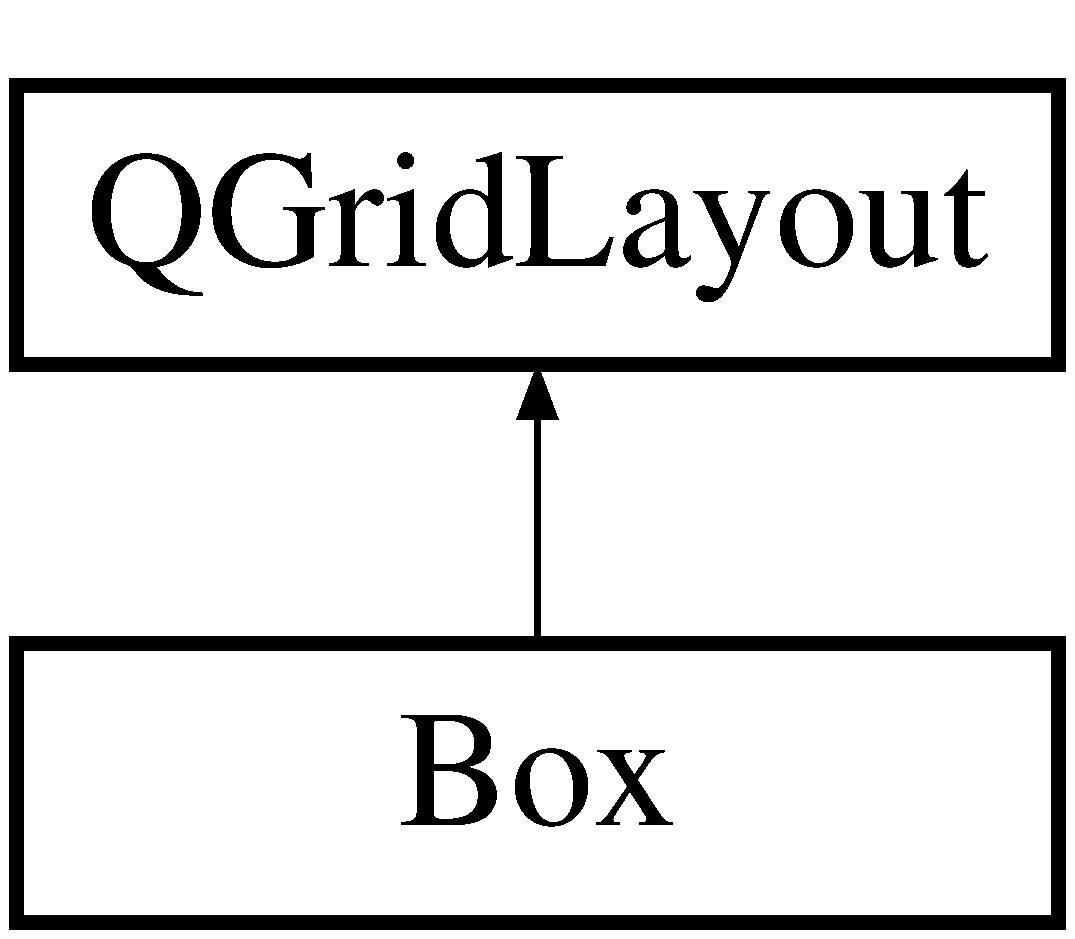
\includegraphics[height=2.000000cm]{class_box}
\end{center}
\end{figure}
\subsection*{Public Member Functions}
\begin{DoxyCompactItemize}
\item 
\mbox{\Hypertarget{class_box_a931e030af8e5656ba81ab96d72854640}\label{class_box_a931e030af8e5656ba81ab96d72854640}} 
{\bfseries Box} (Case my\+Case)
\item 
\mbox{\hyperlink{class_box_ab32e4641d7318dcb3d50779a8089f52e}{Box}} (Case my\+Case, list$<$ Player $>$ players)
\begin{DoxyCompactList}\small\item\em constructeur \mbox{\hyperlink{class_box}{Box}} qui instancie un carre du plateau \end{DoxyCompactList}\item 
int \mbox{\hyperlink{class_box_a253cf157c61db2ca9222d29324387b22}{getX}} () const
\begin{DoxyCompactList}\small\item\em getter de l attribut X. \end{DoxyCompactList}\item 
int \mbox{\hyperlink{class_box_a642cd5e8f8d52529f23df56b9e8acb87}{getY}} () const
\begin{DoxyCompactList}\small\item\em getter de l\textquotesingle{}attribut Y. \end{DoxyCompactList}\item 
void \mbox{\hyperlink{class_box_acd61860cf06c9bad6af1b14f30cd1897}{setX}} (int x)
\begin{DoxyCompactList}\small\item\em setter de l\textquotesingle{}attribut X \end{DoxyCompactList}\item 
void \mbox{\hyperlink{class_box_a35db410e0b63daf638f5d9b43d8aaa59}{setY}} (int y)
\begin{DoxyCompactList}\small\item\em setter de l\textquotesingle{}attribut Y \end{DoxyCompactList}\item 
Q\+Label $\ast$ \mbox{\hyperlink{class_box_aaae920c6f391a06e38e781297ec0b204}{road}} ()
\begin{DoxyCompactList}\small\item\em road chemin pour avoir le box \end{DoxyCompactList}\item 
Objective \mbox{\hyperlink{class_box_a84a5d7227a3ecf4e5d207485b21ff904}{get\+Objective}} () const
\begin{DoxyCompactList}\small\item\em accede a l Objective ds le box \end{DoxyCompactList}\item 
Q\+Label $\ast$ \mbox{\hyperlink{class_box_addada4538ebe16ffd8bef3bb6bf2c83d}{objective}} () const
\begin{DoxyCompactList}\small\item\em objective du box \end{DoxyCompactList}\item 
Q\+Label $\ast$ \mbox{\hyperlink{class_box_abd111ee14102d32764733f0459d691a7}{player\+Blue}} () const
\begin{DoxyCompactList}\small\item\em player\+Blue joueur bleu \end{DoxyCompactList}\item 
Q\+Label $\ast$ \mbox{\hyperlink{class_box_a641488c3839a9825f06aaf4b82ccba32}{player\+Green}} () const
\begin{DoxyCompactList}\small\item\em player\+Green joueur vert \end{DoxyCompactList}\item 
Q\+Label $\ast$ \mbox{\hyperlink{class_box_a4e5e1a2e7f098dddf12db8354c717ecd}{player\+Yellow}} () const
\begin{DoxyCompactList}\small\item\em player\+Yellow joueur jaune \end{DoxyCompactList}\item 
Q\+Label $\ast$ \mbox{\hyperlink{class_box_a2c7957bb93e1d75369c185b23a9b5b1c}{player\+Red}} () const
\begin{DoxyCompactList}\small\item\em player\+Red joueur rouge \end{DoxyCompactList}\item 
Q\+Pixmap \mbox{\hyperlink{class_box_a3db8ad83e6f0562417ce3d9d9b682316}{check\+Objective}} (Objective obj)
\begin{DoxyCompactList}\small\item\em verifie les Objective \end{DoxyCompactList}\item 
void \mbox{\hyperlink{class_box_a5e750fe0b615bb71255701f04975c3e8}{update\+Boxes}} (Case my\+Case, list$<$ Player $>$ players)
\begin{DoxyCompactList}\small\item\em mets a jour les Boxes \end{DoxyCompactList}\item 
void \mbox{\hyperlink{class_box_aec16e613cc17e290448fa203c8968052}{update\+Box}} (Case my\+Case)
\begin{DoxyCompactList}\small\item\em update\+Box \end{DoxyCompactList}\end{DoxyCompactItemize}
\subsection*{Private Attributes}
\begin{DoxyCompactItemize}
\item 
\mbox{\Hypertarget{class_box_a90b4fad8f565e9c815fdba9274cd5fff}\label{class_box_a90b4fad8f565e9c815fdba9274cd5fff}} 
Q\+Label $\ast$ {\bfseries player\+Blue\+\_\+}
\item 
\mbox{\Hypertarget{class_box_a41815b5067adf857cf270318df314e6f}\label{class_box_a41815b5067adf857cf270318df314e6f}} 
Q\+Label $\ast$ {\bfseries player\+Green\+\_\+}
\item 
\mbox{\Hypertarget{class_box_a62b2835ffaacb5ecf0a417fff4228788}\label{class_box_a62b2835ffaacb5ecf0a417fff4228788}} 
Q\+Label $\ast$ {\bfseries player\+Yellow\+\_\+}
\item 
\mbox{\Hypertarget{class_box_a05c0429077d172c1a536f5d5eda386db}\label{class_box_a05c0429077d172c1a536f5d5eda386db}} 
Q\+Label $\ast$ {\bfseries player\+Red\+\_\+}
\item 
\mbox{\Hypertarget{class_box_a380393a9597e2d65fc39b88668acd90f}\label{class_box_a380393a9597e2d65fc39b88668acd90f}} 
Q\+Label $\ast$ {\bfseries road\+\_\+}
\item 
\mbox{\Hypertarget{class_box_a6ff5ee94ced031d1e7da63941408d973}\label{class_box_a6ff5ee94ced031d1e7da63941408d973}} 
Q\+Label $\ast$ {\bfseries objective\+\_\+}
\item 
\mbox{\Hypertarget{class_box_a465d3d1be7534ded22e413416c0d8699}\label{class_box_a465d3d1be7534ded22e413416c0d8699}} 
int {\bfseries x\+Index\+\_\+}
\item 
\mbox{\Hypertarget{class_box_a8da9f43ba66769a8904b5019b334c1a3}\label{class_box_a8da9f43ba66769a8904b5019b334c1a3}} 
int {\bfseries y\+Index\+\_\+}
\item 
\mbox{\Hypertarget{class_box_ac1b9d3c7d4a9b463ce0203b417065af7}\label{class_box_ac1b9d3c7d4a9b463ce0203b417065af7}} 
Q\+Pixmap {\bfseries path\+\_\+}
\item 
\mbox{\Hypertarget{class_box_a3e3d7153ba1eeda72f7584df44e381e9}\label{class_box_a3e3d7153ba1eeda72f7584df44e381e9}} 
Objective {\bfseries obj\+\_\+}
\end{DoxyCompactItemize}


\subsection{Constructor \& Destructor Documentation}
\mbox{\Hypertarget{class_box_ab32e4641d7318dcb3d50779a8089f52e}\label{class_box_ab32e4641d7318dcb3d50779a8089f52e}} 
\index{Box@{Box}!Box@{Box}}
\index{Box@{Box}!Box@{Box}}
\subsubsection{\texorpdfstring{Box()}{Box()}}
{\footnotesize\ttfamily Box\+::\+Box (\begin{DoxyParamCaption}\item[{Case}]{my\+Case,  }\item[{list$<$ Player $>$}]{players }\end{DoxyParamCaption})}



constructeur \mbox{\hyperlink{class_box}{Box}} qui instancie un carre du plateau 


\begin{DoxyParams}{Parameters}
{\em my\+Case} & \\
\hline
{\em players} & \\
\hline
\end{DoxyParams}


\subsection{Member Function Documentation}
\mbox{\Hypertarget{class_box_a3db8ad83e6f0562417ce3d9d9b682316}\label{class_box_a3db8ad83e6f0562417ce3d9d9b682316}} 
\index{Box@{Box}!check\+Objective@{check\+Objective}}
\index{check\+Objective@{check\+Objective}!Box@{Box}}
\subsubsection{\texorpdfstring{check\+Objective()}{checkObjective()}}
{\footnotesize\ttfamily Q\+Pixmap Box\+::check\+Objective (\begin{DoxyParamCaption}\item[{Objective}]{obj }\end{DoxyParamCaption})}



verifie les Objective 


\begin{DoxyParams}{Parameters}
{\em obj} & \\
\hline
\end{DoxyParams}
\begin{DoxyReturn}{Returns}

\end{DoxyReturn}
\mbox{\Hypertarget{class_box_a84a5d7227a3ecf4e5d207485b21ff904}\label{class_box_a84a5d7227a3ecf4e5d207485b21ff904}} 
\index{Box@{Box}!get\+Objective@{get\+Objective}}
\index{get\+Objective@{get\+Objective}!Box@{Box}}
\subsubsection{\texorpdfstring{get\+Objective()}{getObjective()}}
{\footnotesize\ttfamily Objective Box\+::get\+Objective (\begin{DoxyParamCaption}{ }\end{DoxyParamCaption}) const\hspace{0.3cm}{\ttfamily [inline]}}



accede a l Objective ds le box 

\begin{DoxyReturn}{Returns}

\end{DoxyReturn}
\mbox{\Hypertarget{class_box_a253cf157c61db2ca9222d29324387b22}\label{class_box_a253cf157c61db2ca9222d29324387b22}} 
\index{Box@{Box}!getX@{getX}}
\index{getX@{getX}!Box@{Box}}
\subsubsection{\texorpdfstring{get\+X()}{getX()}}
{\footnotesize\ttfamily Box\+::getX (\begin{DoxyParamCaption}{ }\end{DoxyParamCaption}) const\hspace{0.3cm}{\ttfamily [inline]}}



getter de l attribut X. 

\begin{DoxyReturn}{Returns}
le X trouver. 
\end{DoxyReturn}
\mbox{\Hypertarget{class_box_a642cd5e8f8d52529f23df56b9e8acb87}\label{class_box_a642cd5e8f8d52529f23df56b9e8acb87}} 
\index{Box@{Box}!getY@{getY}}
\index{getY@{getY}!Box@{Box}}
\subsubsection{\texorpdfstring{get\+Y()}{getY()}}
{\footnotesize\ttfamily Box\+::getY (\begin{DoxyParamCaption}{ }\end{DoxyParamCaption}) const\hspace{0.3cm}{\ttfamily [inline]}}



getter de l\textquotesingle{}attribut Y. 

\begin{DoxyReturn}{Returns}
le Y trouver 
\end{DoxyReturn}
\mbox{\Hypertarget{class_box_addada4538ebe16ffd8bef3bb6bf2c83d}\label{class_box_addada4538ebe16ffd8bef3bb6bf2c83d}} 
\index{Box@{Box}!objective@{objective}}
\index{objective@{objective}!Box@{Box}}
\subsubsection{\texorpdfstring{objective()}{objective()}}
{\footnotesize\ttfamily Q\+Label $\ast$ Box\+::objective (\begin{DoxyParamCaption}{ }\end{DoxyParamCaption}) const\hspace{0.3cm}{\ttfamily [inline]}}



objective du box 

\begin{DoxyReturn}{Returns}

\end{DoxyReturn}
\mbox{\Hypertarget{class_box_abd111ee14102d32764733f0459d691a7}\label{class_box_abd111ee14102d32764733f0459d691a7}} 
\index{Box@{Box}!player\+Blue@{player\+Blue}}
\index{player\+Blue@{player\+Blue}!Box@{Box}}
\subsubsection{\texorpdfstring{player\+Blue()}{playerBlue()}}
{\footnotesize\ttfamily Q\+Label $\ast$ Box\+::player\+Blue (\begin{DoxyParamCaption}{ }\end{DoxyParamCaption}) const\hspace{0.3cm}{\ttfamily [inline]}}



player\+Blue joueur bleu 

\begin{DoxyReturn}{Returns}
un label 
\end{DoxyReturn}
\mbox{\Hypertarget{class_box_a641488c3839a9825f06aaf4b82ccba32}\label{class_box_a641488c3839a9825f06aaf4b82ccba32}} 
\index{Box@{Box}!player\+Green@{player\+Green}}
\index{player\+Green@{player\+Green}!Box@{Box}}
\subsubsection{\texorpdfstring{player\+Green()}{playerGreen()}}
{\footnotesize\ttfamily Q\+Label $\ast$ Box\+::player\+Green (\begin{DoxyParamCaption}{ }\end{DoxyParamCaption}) const\hspace{0.3cm}{\ttfamily [inline]}}



player\+Green joueur vert 

\begin{DoxyReturn}{Returns}
un label 
\end{DoxyReturn}
\mbox{\Hypertarget{class_box_a2c7957bb93e1d75369c185b23a9b5b1c}\label{class_box_a2c7957bb93e1d75369c185b23a9b5b1c}} 
\index{Box@{Box}!player\+Red@{player\+Red}}
\index{player\+Red@{player\+Red}!Box@{Box}}
\subsubsection{\texorpdfstring{player\+Red()}{playerRed()}}
{\footnotesize\ttfamily Q\+Label $\ast$ Box\+::player\+Red (\begin{DoxyParamCaption}{ }\end{DoxyParamCaption}) const\hspace{0.3cm}{\ttfamily [inline]}}



player\+Red joueur rouge 

\begin{DoxyReturn}{Returns}
un label 
\end{DoxyReturn}
\mbox{\Hypertarget{class_box_a4e5e1a2e7f098dddf12db8354c717ecd}\label{class_box_a4e5e1a2e7f098dddf12db8354c717ecd}} 
\index{Box@{Box}!player\+Yellow@{player\+Yellow}}
\index{player\+Yellow@{player\+Yellow}!Box@{Box}}
\subsubsection{\texorpdfstring{player\+Yellow()}{playerYellow()}}
{\footnotesize\ttfamily Q\+Label $\ast$ Box\+::player\+Yellow (\begin{DoxyParamCaption}{ }\end{DoxyParamCaption}) const\hspace{0.3cm}{\ttfamily [inline]}}



player\+Yellow joueur jaune 

\begin{DoxyReturn}{Returns}
un label 
\end{DoxyReturn}
\mbox{\Hypertarget{class_box_aaae920c6f391a06e38e781297ec0b204}\label{class_box_aaae920c6f391a06e38e781297ec0b204}} 
\index{Box@{Box}!road@{road}}
\index{road@{road}!Box@{Box}}
\subsubsection{\texorpdfstring{road()}{road()}}
{\footnotesize\ttfamily Q\+Label $\ast$ Box\+::road (\begin{DoxyParamCaption}{ }\end{DoxyParamCaption})\hspace{0.3cm}{\ttfamily [inline]}}



road chemin pour avoir le box 

\begin{DoxyReturn}{Returns}

\end{DoxyReturn}
\mbox{\Hypertarget{class_box_acd61860cf06c9bad6af1b14f30cd1897}\label{class_box_acd61860cf06c9bad6af1b14f30cd1897}} 
\index{Box@{Box}!setX@{setX}}
\index{setX@{setX}!Box@{Box}}
\subsubsection{\texorpdfstring{set\+X()}{setX()}}
{\footnotesize\ttfamily void Box\+::setX (\begin{DoxyParamCaption}\item[{int}]{x }\end{DoxyParamCaption})\hspace{0.3cm}{\ttfamily [inline]}}



setter de l\textquotesingle{}attribut X 


\begin{DoxyParams}{Parameters}
{\em valeur} & fournie de x a changer \\
\hline
\end{DoxyParams}
\mbox{\Hypertarget{class_box_a35db410e0b63daf638f5d9b43d8aaa59}\label{class_box_a35db410e0b63daf638f5d9b43d8aaa59}} 
\index{Box@{Box}!setY@{setY}}
\index{setY@{setY}!Box@{Box}}
\subsubsection{\texorpdfstring{set\+Y()}{setY()}}
{\footnotesize\ttfamily void Box\+::setY (\begin{DoxyParamCaption}\item[{int}]{y }\end{DoxyParamCaption})\hspace{0.3cm}{\ttfamily [inline]}}



setter de l\textquotesingle{}attribut Y 


\begin{DoxyParams}{Parameters}
{\em valeur} & fournie de y a changer \\
\hline
\end{DoxyParams}
\mbox{\Hypertarget{class_box_aec16e613cc17e290448fa203c8968052}\label{class_box_aec16e613cc17e290448fa203c8968052}} 
\index{Box@{Box}!update\+Box@{update\+Box}}
\index{update\+Box@{update\+Box}!Box@{Box}}
\subsubsection{\texorpdfstring{update\+Box()}{updateBox()}}
{\footnotesize\ttfamily void Box\+::update\+Box (\begin{DoxyParamCaption}\item[{Case}]{my\+Case }\end{DoxyParamCaption})}



update\+Box 


\begin{DoxyParams}{Parameters}
{\em my\+Case} & \\
\hline
\end{DoxyParams}
\mbox{\Hypertarget{class_box_a5e750fe0b615bb71255701f04975c3e8}\label{class_box_a5e750fe0b615bb71255701f04975c3e8}} 
\index{Box@{Box}!update\+Boxes@{update\+Boxes}}
\index{update\+Boxes@{update\+Boxes}!Box@{Box}}
\subsubsection{\texorpdfstring{update\+Boxes()}{updateBoxes()}}
{\footnotesize\ttfamily void Box\+::update\+Boxes (\begin{DoxyParamCaption}\item[{Case}]{my\+Case,  }\item[{list$<$ Player $>$}]{players }\end{DoxyParamCaption})}



mets a jour les Boxes 


\begin{DoxyParams}{Parameters}
{\em my\+Case} & \\
\hline
{\em players} & \\
\hline
\end{DoxyParams}


The documentation for this class was generated from the following files\+:\begin{DoxyCompactItemize}
\item 
C\+:/\+Users/benaz/\+Documents/cpp+/\+Labyrinth\+Project/box.\+h\item 
C\+:/\+Users/benaz/\+Documents/cpp+/\+Labyrinth\+Project/box.\+cpp\end{DoxyCompactItemize}

\hypertarget{classnvs_1_1_observer}{}\section{nvs\+:\+:Observer Class Reference}
\label{classnvs_1_1_observer}\index{nvs\+::\+Observer@{nvs\+::\+Observer}}


Classe abstraite de base de tout observateur.  




{\ttfamily \#include $<$observer.\+h$>$}

Inheritance diagram for nvs\+:\+:Observer\+:\begin{figure}[H]
\begin{center}
\leavevmode
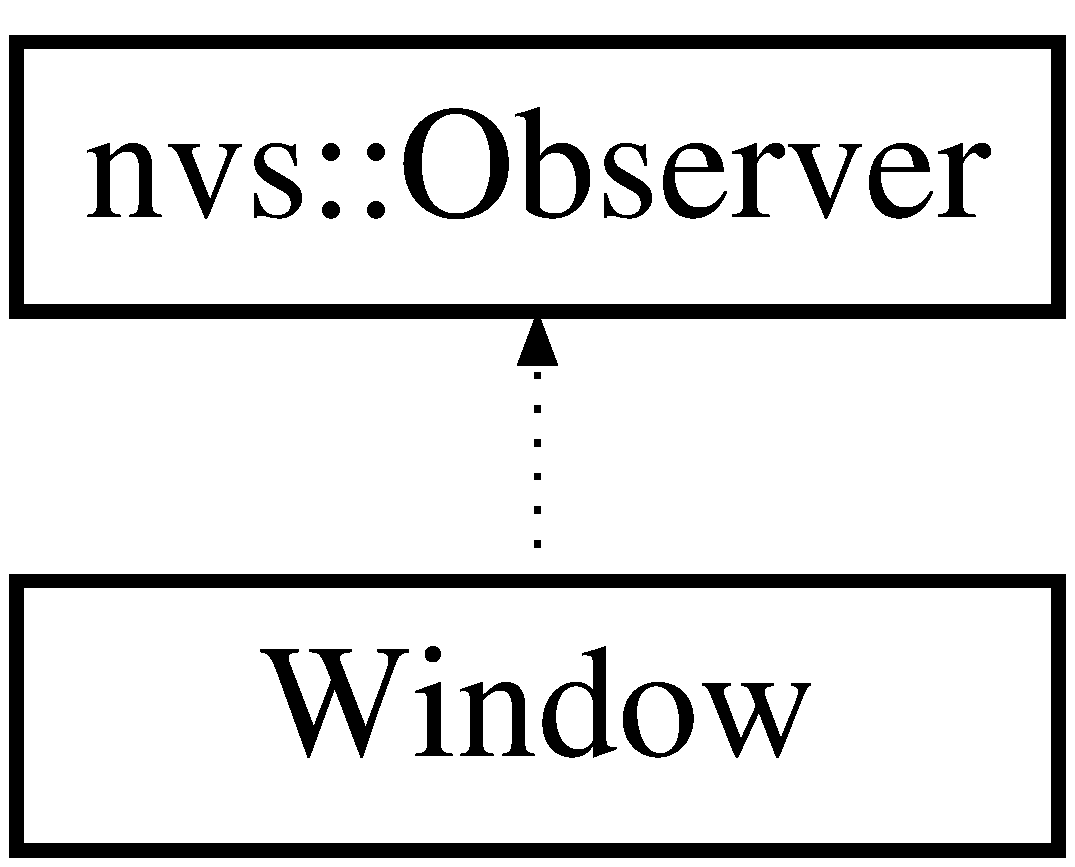
\includegraphics[height=2.000000cm]{classnvs_1_1_observer}
\end{center}
\end{figure}
\subsection*{Public Member Functions}
\begin{DoxyCompactItemize}
\item 
virtual void \mbox{\hyperlink{classnvs_1_1_observer_a4c0373c644180bdc48558e5248968b3a}{update}} (const \mbox{\hyperlink{classnvs_1_1_subject}{Subject}} $\ast$subject)=0
\begin{DoxyCompactList}\small\item\em Méthode virtuelle pure que chaque observateur concret doit implémenter \+: c\textquotesingle{}est cette méthode qu\textquotesingle{}appelle le sujet observé lors d\textquotesingle{}une notification. \end{DoxyCompactList}\item 
\mbox{\Hypertarget{classnvs_1_1_observer_aad2df366134bc340a8717360cd7307d2}\label{classnvs_1_1_observer_aad2df366134bc340a8717360cd7307d2}} 
virtual \mbox{\hyperlink{classnvs_1_1_observer_aad2df366134bc340a8717360cd7307d2}{$\sim$\+Observer}} ()=default
\begin{DoxyCompactList}\small\item\em Destructeur virtuel par défaut car utilisation polymorphique. \end{DoxyCompactList}\item 
\mbox{\hyperlink{classnvs_1_1_observer_a4515f485c0ca822e088cffdfc30d3ed8}{Observer}} (const \mbox{\hyperlink{classnvs_1_1_observer}{Observer}} \&)=default
\begin{DoxyCompactList}\small\item\em Constructeur par recopie par défaut. \end{DoxyCompactList}\item 
\mbox{\hyperlink{classnvs_1_1_observer_a3058c1a0d319e92a563a6ed09354e8f6}{Observer}} (\mbox{\hyperlink{classnvs_1_1_observer}{Observer}} \&\&)=default
\begin{DoxyCompactList}\small\item\em Constructeur par déplacement par défaut. \end{DoxyCompactList}\item 
\mbox{\hyperlink{classnvs_1_1_observer}{Observer}} \& \mbox{\hyperlink{classnvs_1_1_observer_a405218b4689360fb9d8fdab3bed37dad}{operator=}} (const \mbox{\hyperlink{classnvs_1_1_observer}{Observer}} \&)=default
\begin{DoxyCompactList}\small\item\em Opérateur d\textquotesingle{}assignation par recopie par défaut. \end{DoxyCompactList}\item 
\mbox{\hyperlink{classnvs_1_1_observer}{Observer}} \& \mbox{\hyperlink{classnvs_1_1_observer_a12803c6d97f98c355a0f46b36a35d64b}{operator=}} (\mbox{\hyperlink{classnvs_1_1_observer}{Observer}} \&\&)=default
\begin{DoxyCompactList}\small\item\em Opérateur d\textquotesingle{}assignation par déplacement par défaut. \end{DoxyCompactList}\end{DoxyCompactItemize}
\subsection*{Protected Member Functions}
\begin{DoxyCompactItemize}
\item 
\mbox{\hyperlink{classnvs_1_1_observer_a755ac6084a75b80cf8b7a7cf6fd4e8dd}{Observer}} ()=default
\begin{DoxyCompactList}\small\item\em Constructeur protégé pour éviter l\textquotesingle{}instanciation hors héritage. \end{DoxyCompactList}\end{DoxyCompactItemize}


\subsection{Detailed Description}
Classe abstraite de base de tout observateur. 

Classe dont dérive tout écouteur (ou \char`\"{}observateur\char`\"{}) du modèle de conception \char`\"{}\+Observateur / Sujet\+D\+Observation\char`\"{}.

\begin{DoxySeeAlso}{See also}
\mbox{\hyperlink{classnvs_1_1_subject}{Subject}}. 

\href{https://en.wikipedia.org/wiki/Observer_pattern}{\tt https\+://en.\+wikipedia.\+org/wiki/\+Observer\+\_\+pattern} 
\end{DoxySeeAlso}


\subsection{Constructor \& Destructor Documentation}
\mbox{\Hypertarget{classnvs_1_1_observer_a4515f485c0ca822e088cffdfc30d3ed8}\label{classnvs_1_1_observer_a4515f485c0ca822e088cffdfc30d3ed8}} 
\index{nvs\+::\+Observer@{nvs\+::\+Observer}!Observer@{Observer}}
\index{Observer@{Observer}!nvs\+::\+Observer@{nvs\+::\+Observer}}
\subsubsection{\texorpdfstring{Observer()}{Observer()}\hspace{0.1cm}{\footnotesize\ttfamily [1/3]}}
{\footnotesize\ttfamily nvs\+::\+Observer\+::\+Observer (\begin{DoxyParamCaption}\item[{const \mbox{\hyperlink{classnvs_1_1_observer}{Observer}} \&}]{ }\end{DoxyParamCaption})\hspace{0.3cm}{\ttfamily [default]}}



Constructeur par recopie par défaut. 

Le destructeur virtuel par défaut a des effets en cascade.

\begin{DoxySeeAlso}{See also}
\href{http://stackoverflow.com/q/33957037}{\tt http\+://stackoverflow.\+com/q/33957037} 

\href{http://scottmeyers.blogspot.de/2014/03/a-concern-about-rule-of-zero.html}{\tt http\+://scottmeyers.\+blogspot.\+de/2014/03/a-\/concern-\/about-\/rule-\/of-\/zero.\+html} 

\href{https://blog.feabhas.com/2015/11/becoming-a-rule-of-zero-hero/}{\tt https\+://blog.\+feabhas.\+com/2015/11/becoming-\/a-\/rule-\/of-\/zero-\/hero/} 
\end{DoxySeeAlso}
\mbox{\Hypertarget{classnvs_1_1_observer_a3058c1a0d319e92a563a6ed09354e8f6}\label{classnvs_1_1_observer_a3058c1a0d319e92a563a6ed09354e8f6}} 
\index{nvs\+::\+Observer@{nvs\+::\+Observer}!Observer@{Observer}}
\index{Observer@{Observer}!nvs\+::\+Observer@{nvs\+::\+Observer}}
\subsubsection{\texorpdfstring{Observer()}{Observer()}\hspace{0.1cm}{\footnotesize\ttfamily [2/3]}}
{\footnotesize\ttfamily nvs\+::\+Observer\+::\+Observer (\begin{DoxyParamCaption}\item[{\mbox{\hyperlink{classnvs_1_1_observer}{Observer}} \&\&}]{ }\end{DoxyParamCaption})\hspace{0.3cm}{\ttfamily [default]}}



Constructeur par déplacement par défaut. 

Le destructeur virtuel par défaut a des effets en cascade.

\begin{DoxySeeAlso}{See also}
\href{http://stackoverflow.com/q/33957037}{\tt http\+://stackoverflow.\+com/q/33957037} 

\href{http://scottmeyers.blogspot.de/2014/03/a-concern-about-rule-of-zero.html}{\tt http\+://scottmeyers.\+blogspot.\+de/2014/03/a-\/concern-\/about-\/rule-\/of-\/zero.\+html} 

\href{https://blog.feabhas.com/2015/11/becoming-a-rule-of-zero-hero/}{\tt https\+://blog.\+feabhas.\+com/2015/11/becoming-\/a-\/rule-\/of-\/zero-\/hero/} 
\end{DoxySeeAlso}
\mbox{\Hypertarget{classnvs_1_1_observer_a755ac6084a75b80cf8b7a7cf6fd4e8dd}\label{classnvs_1_1_observer_a755ac6084a75b80cf8b7a7cf6fd4e8dd}} 
\index{nvs\+::\+Observer@{nvs\+::\+Observer}!Observer@{Observer}}
\index{Observer@{Observer}!nvs\+::\+Observer@{nvs\+::\+Observer}}
\subsubsection{\texorpdfstring{Observer()}{Observer()}\hspace{0.1cm}{\footnotesize\ttfamily [3/3]}}
{\footnotesize\ttfamily nvs\+::\+Observer\+::\+Observer (\begin{DoxyParamCaption}{ }\end{DoxyParamCaption})\hspace{0.3cm}{\ttfamily [protected]}, {\ttfamily [default]}}



Constructeur protégé pour éviter l\textquotesingle{}instanciation hors héritage. 

Le destructeur virtuel par défaut a des effets en cascade.

\begin{DoxySeeAlso}{See also}
\href{http://stackoverflow.com/q/33957037}{\tt http\+://stackoverflow.\+com/q/33957037} 

\href{http://scottmeyers.blogspot.de/2014/03/a-concern-about-rule-of-zero.html}{\tt http\+://scottmeyers.\+blogspot.\+de/2014/03/a-\/concern-\/about-\/rule-\/of-\/zero.\+html} 

\href{https://blog.feabhas.com/2015/11/becoming-a-rule-of-zero-hero/}{\tt https\+://blog.\+feabhas.\+com/2015/11/becoming-\/a-\/rule-\/of-\/zero-\/hero/} 
\end{DoxySeeAlso}


\subsection{Member Function Documentation}
\mbox{\Hypertarget{classnvs_1_1_observer_a405218b4689360fb9d8fdab3bed37dad}\label{classnvs_1_1_observer_a405218b4689360fb9d8fdab3bed37dad}} 
\index{nvs\+::\+Observer@{nvs\+::\+Observer}!operator=@{operator=}}
\index{operator=@{operator=}!nvs\+::\+Observer@{nvs\+::\+Observer}}
\subsubsection{\texorpdfstring{operator=()}{operator=()}\hspace{0.1cm}{\footnotesize\ttfamily [1/2]}}
{\footnotesize\ttfamily \mbox{\hyperlink{classnvs_1_1_observer}{Observer}}\& nvs\+::\+Observer\+::operator= (\begin{DoxyParamCaption}\item[{const \mbox{\hyperlink{classnvs_1_1_observer}{Observer}} \&}]{ }\end{DoxyParamCaption})\hspace{0.3cm}{\ttfamily [default]}}



Opérateur d\textquotesingle{}assignation par recopie par défaut. 

Le destructeur virtuel par défaut a des effets en cascade.

\begin{DoxySeeAlso}{See also}
\href{http://stackoverflow.com/q/33957037}{\tt http\+://stackoverflow.\+com/q/33957037} 

\href{http://scottmeyers.blogspot.de/2014/03/a-concern-about-rule-of-zero.html}{\tt http\+://scottmeyers.\+blogspot.\+de/2014/03/a-\/concern-\/about-\/rule-\/of-\/zero.\+html} 

\href{https://blog.feabhas.com/2015/11/becoming-a-rule-of-zero-hero/}{\tt https\+://blog.\+feabhas.\+com/2015/11/becoming-\/a-\/rule-\/of-\/zero-\/hero/} 
\end{DoxySeeAlso}
\mbox{\Hypertarget{classnvs_1_1_observer_a12803c6d97f98c355a0f46b36a35d64b}\label{classnvs_1_1_observer_a12803c6d97f98c355a0f46b36a35d64b}} 
\index{nvs\+::\+Observer@{nvs\+::\+Observer}!operator=@{operator=}}
\index{operator=@{operator=}!nvs\+::\+Observer@{nvs\+::\+Observer}}
\subsubsection{\texorpdfstring{operator=()}{operator=()}\hspace{0.1cm}{\footnotesize\ttfamily [2/2]}}
{\footnotesize\ttfamily \mbox{\hyperlink{classnvs_1_1_observer}{Observer}}\& nvs\+::\+Observer\+::operator= (\begin{DoxyParamCaption}\item[{\mbox{\hyperlink{classnvs_1_1_observer}{Observer}} \&\&}]{ }\end{DoxyParamCaption})\hspace{0.3cm}{\ttfamily [default]}}



Opérateur d\textquotesingle{}assignation par déplacement par défaut. 

Le destructeur virtuel par défaut a des effets en cascade.

\begin{DoxySeeAlso}{See also}
\href{http://stackoverflow.com/q/33957037}{\tt http\+://stackoverflow.\+com/q/33957037} 

\href{http://scottmeyers.blogspot.de/2014/03/a-concern-about-rule-of-zero.html}{\tt http\+://scottmeyers.\+blogspot.\+de/2014/03/a-\/concern-\/about-\/rule-\/of-\/zero.\+html} 

\href{https://blog.feabhas.com/2015/11/becoming-a-rule-of-zero-hero/}{\tt https\+://blog.\+feabhas.\+com/2015/11/becoming-\/a-\/rule-\/of-\/zero-\/hero/} 
\end{DoxySeeAlso}
\mbox{\Hypertarget{classnvs_1_1_observer_a4c0373c644180bdc48558e5248968b3a}\label{classnvs_1_1_observer_a4c0373c644180bdc48558e5248968b3a}} 
\index{nvs\+::\+Observer@{nvs\+::\+Observer}!update@{update}}
\index{update@{update}!nvs\+::\+Observer@{nvs\+::\+Observer}}
\subsubsection{\texorpdfstring{update()}{update()}}
{\footnotesize\ttfamily virtual void nvs\+::\+Observer\+::update (\begin{DoxyParamCaption}\item[{const \mbox{\hyperlink{classnvs_1_1_subject}{Subject}} $\ast$}]{subject }\end{DoxyParamCaption})\hspace{0.3cm}{\ttfamily [pure virtual]}}



Méthode virtuelle pure que chaque observateur concret doit implémenter \+: c\textquotesingle{}est cette méthode qu\textquotesingle{}appelle le sujet observé lors d\textquotesingle{}une notification. 


\begin{DoxyParams}{Parameters}
{\em subject} & le sujet d\textquotesingle{}observation qui notifie un changement. \\
\hline
\end{DoxyParams}
\begin{DoxySeeAlso}{See also}
\mbox{\hyperlink{classnvs_1_1_subject_ac0c7f6fc31ec3dd61c1e102cb565cdf9}{Subject\+::notify\+Observers()}}. 
\end{DoxySeeAlso}


Implemented in \mbox{\hyperlink{class_window_affdeb2564502d9f4ca63e8c0c0c6f7c0}{Window}}.



The documentation for this class was generated from the following file\+:\begin{DoxyCompactItemize}
\item 
C\+:/\+Users/benaz/\+Documents/cpp+/\+Labyrinth\+Project/\mbox{\hyperlink{observer_8h}{observer.\+h}}\end{DoxyCompactItemize}

\hypertarget{classnvs_1_1_subject}{}\section{nvs\+:\+:Subject Class Reference}
\label{classnvs_1_1_subject}\index{nvs\+::\+Subject@{nvs\+::\+Subject}}


Classe de base de tout \char`\"{}sujet d\textquotesingle{}observation\char`\"{}.  




{\ttfamily \#include $<$subject.\+h$>$}

\subsection*{Public Member Functions}
\begin{DoxyCompactItemize}
\item 
\mbox{\Hypertarget{classnvs_1_1_subject_ae6c2083563615d4f449f55b970835816}\label{classnvs_1_1_subject_ae6c2083563615d4f449f55b970835816}} 
virtual \mbox{\hyperlink{classnvs_1_1_subject_ae6c2083563615d4f449f55b970835816}{$\sim$\+Subject}} ()=default
\begin{DoxyCompactList}\small\item\em Destructeur virtuel par défaut car utilisation polymorphique. \end{DoxyCompactList}\item 
\mbox{\hyperlink{classnvs_1_1_subject_acb8bf74c98c8ec96d999ce98cd3fab22}{Subject}} (const \mbox{\hyperlink{classnvs_1_1_subject}{Subject}} \&)=default
\begin{DoxyCompactList}\small\item\em Constructeur par recopie par défaut. \end{DoxyCompactList}\item 
\mbox{\hyperlink{classnvs_1_1_subject_a228776e466dd330075d3f4a089c006f4}{Subject}} (\mbox{\hyperlink{classnvs_1_1_subject}{Subject}} \&\&)=default
\begin{DoxyCompactList}\small\item\em Constructeur par déplacement par défaut. \end{DoxyCompactList}\item 
\mbox{\hyperlink{classnvs_1_1_subject}{Subject}} \& \mbox{\hyperlink{classnvs_1_1_subject_aba16a1e0481f97b74a66468dab1d50bf}{operator=}} (const \mbox{\hyperlink{classnvs_1_1_subject}{Subject}} \&)=default
\begin{DoxyCompactList}\small\item\em Opérateur d\textquotesingle{}assignation par recopie par défaut. \end{DoxyCompactList}\item 
\mbox{\hyperlink{classnvs_1_1_subject}{Subject}} \& \mbox{\hyperlink{classnvs_1_1_subject_afa3849e579c73fc54258f2b5ddd8317e}{operator=}} (\mbox{\hyperlink{classnvs_1_1_subject}{Subject}} \&\&)=default
\begin{DoxyCompactList}\small\item\em Opérateur d\textquotesingle{}assignation par déplacement par défaut. \end{DoxyCompactList}\item 
virtual void \mbox{\hyperlink{classnvs_1_1_subject_a4a476a25d1fa0db77f5ca86a6b0637f2}{register\+Observer}} (\mbox{\hyperlink{classnvs_1_1_observer}{Observer}} $\ast$observer) final
\begin{DoxyCompactList}\small\item\em Méthode permettant à un observateur de s\textquotesingle{}enregistrer comme écouteur du sujet d\textquotesingle{}observation. \end{DoxyCompactList}\item 
virtual void \mbox{\hyperlink{classnvs_1_1_subject_a749bc5b9a58ba0f72abbbce0f01f8a24}{unregister\+Observer}} (\mbox{\hyperlink{classnvs_1_1_observer}{Observer}} $\ast$observer) final
\begin{DoxyCompactList}\small\item\em Méthode permettant à un observateur de se retirer de la liste des écouteurs patentés du sujet d\textquotesingle{}observation. \end{DoxyCompactList}\end{DoxyCompactItemize}
\subsection*{Protected Member Functions}
\begin{DoxyCompactItemize}
\item 
\mbox{\Hypertarget{classnvs_1_1_subject_a698aabcd0083be40995673ba4d887487}\label{classnvs_1_1_subject_a698aabcd0083be40995673ba4d887487}} 
\mbox{\hyperlink{classnvs_1_1_subject_a698aabcd0083be40995673ba4d887487}{Subject}} ()=default
\begin{DoxyCompactList}\small\item\em Constructeur protégé pour éviter l\textquotesingle{}instanciation hors héritage. \end{DoxyCompactList}\item 
virtual void \mbox{\hyperlink{classnvs_1_1_subject_ac0c7f6fc31ec3dd61c1e102cb565cdf9}{notify\+Observers}} () const final
\begin{DoxyCompactList}\small\item\em Méthode qui se charge de prévenir les observateurs d\textquotesingle{}un changement d\textquotesingle{}état du sujet d\textquotesingle{}observation, en invoquant leur méthode \mbox{\hyperlink{classnvs_1_1_observer_a4c0373c644180bdc48558e5248968b3a}{Observer\+::update()}}. \end{DoxyCompactList}\end{DoxyCompactItemize}
\subsection*{Protected Attributes}
\begin{DoxyCompactItemize}
\item 
\mbox{\Hypertarget{classnvs_1_1_subject_a71448bb8a51b098168d010dfe854450c}\label{classnvs_1_1_subject_a71448bb8a51b098168d010dfe854450c}} 
std\+::set$<$ \mbox{\hyperlink{classnvs_1_1_observer}{Observer}} $\ast$ $>$ \mbox{\hyperlink{classnvs_1_1_subject_a71448bb8a51b098168d010dfe854450c}{observers\+\_\+}} \{ \}
\begin{DoxyCompactList}\small\item\em L\textquotesingle{}ensemble d\textquotesingle{}observateurs enregistrés. \end{DoxyCompactList}\end{DoxyCompactItemize}


\subsection{Detailed Description}
Classe de base de tout \char`\"{}sujet d\textquotesingle{}observation\char`\"{}. 

Classe dont dérive toute source d\textquotesingle{}événement (ou \char`\"{}sujet d\textquotesingle{}observation\char`\"{}) du modèle de conception \char`\"{}\+Observateur / Sujet\+D\+Observation\char`\"{}.

\begin{DoxySeeAlso}{See also}
\mbox{\hyperlink{classnvs_1_1_observer}{Observer}}. 
\end{DoxySeeAlso}


\subsection{Constructor \& Destructor Documentation}
\mbox{\Hypertarget{classnvs_1_1_subject_acb8bf74c98c8ec96d999ce98cd3fab22}\label{classnvs_1_1_subject_acb8bf74c98c8ec96d999ce98cd3fab22}} 
\index{nvs\+::\+Subject@{nvs\+::\+Subject}!Subject@{Subject}}
\index{Subject@{Subject}!nvs\+::\+Subject@{nvs\+::\+Subject}}
\subsubsection{\texorpdfstring{Subject()}{Subject()}\hspace{0.1cm}{\footnotesize\ttfamily [1/2]}}
{\footnotesize\ttfamily nvs\+::\+Subject\+::\+Subject (\begin{DoxyParamCaption}\item[{const \mbox{\hyperlink{classnvs_1_1_subject}{Subject}} \&}]{ }\end{DoxyParamCaption})\hspace{0.3cm}{\ttfamily [default]}}



Constructeur par recopie par défaut. 

Le destructeur virtuel par défaut a des effets en cascade.

\begin{DoxySeeAlso}{See also}
\href{http://stackoverflow.com/q/33957037}{\tt http\+://stackoverflow.\+com/q/33957037} 

\href{http://scottmeyers.blogspot.de/2014/03/a-concern-about-rule-of-zero.html}{\tt http\+://scottmeyers.\+blogspot.\+de/2014/03/a-\/concern-\/about-\/rule-\/of-\/zero.\+html} 

\href{https://blog.feabhas.com/2015/11/becoming-a-rule-of-zero-hero/}{\tt https\+://blog.\+feabhas.\+com/2015/11/becoming-\/a-\/rule-\/of-\/zero-\/hero/} 
\end{DoxySeeAlso}
\mbox{\Hypertarget{classnvs_1_1_subject_a228776e466dd330075d3f4a089c006f4}\label{classnvs_1_1_subject_a228776e466dd330075d3f4a089c006f4}} 
\index{nvs\+::\+Subject@{nvs\+::\+Subject}!Subject@{Subject}}
\index{Subject@{Subject}!nvs\+::\+Subject@{nvs\+::\+Subject}}
\subsubsection{\texorpdfstring{Subject()}{Subject()}\hspace{0.1cm}{\footnotesize\ttfamily [2/2]}}
{\footnotesize\ttfamily nvs\+::\+Subject\+::\+Subject (\begin{DoxyParamCaption}\item[{\mbox{\hyperlink{classnvs_1_1_subject}{Subject}} \&\&}]{ }\end{DoxyParamCaption})\hspace{0.3cm}{\ttfamily [default]}}



Constructeur par déplacement par défaut. 

Le destructeur virtuel par défaut a des effets en cascade.

\begin{DoxySeeAlso}{See also}
\href{http://stackoverflow.com/q/33957037}{\tt http\+://stackoverflow.\+com/q/33957037} 

\href{http://scottmeyers.blogspot.de/2014/03/a-concern-about-rule-of-zero.html}{\tt http\+://scottmeyers.\+blogspot.\+de/2014/03/a-\/concern-\/about-\/rule-\/of-\/zero.\+html} 

\href{https://blog.feabhas.com/2015/11/becoming-a-rule-of-zero-hero/}{\tt https\+://blog.\+feabhas.\+com/2015/11/becoming-\/a-\/rule-\/of-\/zero-\/hero/} 
\end{DoxySeeAlso}


\subsection{Member Function Documentation}
\mbox{\Hypertarget{classnvs_1_1_subject_ac0c7f6fc31ec3dd61c1e102cb565cdf9}\label{classnvs_1_1_subject_ac0c7f6fc31ec3dd61c1e102cb565cdf9}} 
\index{nvs\+::\+Subject@{nvs\+::\+Subject}!notify\+Observers@{notify\+Observers}}
\index{notify\+Observers@{notify\+Observers}!nvs\+::\+Subject@{nvs\+::\+Subject}}
\subsubsection{\texorpdfstring{notify\+Observers()}{notifyObservers()}}
{\footnotesize\ttfamily void nvs\+::\+Subject\+::notify\+Observers (\begin{DoxyParamCaption}{ }\end{DoxyParamCaption}) const\hspace{0.3cm}{\ttfamily [final]}, {\ttfamily [protected]}, {\ttfamily [virtual]}}



Méthode qui se charge de prévenir les observateurs d\textquotesingle{}un changement d\textquotesingle{}état du sujet d\textquotesingle{}observation, en invoquant leur méthode \mbox{\hyperlink{classnvs_1_1_observer_a4c0373c644180bdc48558e5248968b3a}{Observer\+::update()}}. 

\begin{DoxySeeAlso}{See also}
\mbox{\hyperlink{classnvs_1_1_observer_a4c0373c644180bdc48558e5248968b3a}{Observer\+::update(const Subject $\ast$)}}. 
\end{DoxySeeAlso}
\mbox{\Hypertarget{classnvs_1_1_subject_aba16a1e0481f97b74a66468dab1d50bf}\label{classnvs_1_1_subject_aba16a1e0481f97b74a66468dab1d50bf}} 
\index{nvs\+::\+Subject@{nvs\+::\+Subject}!operator=@{operator=}}
\index{operator=@{operator=}!nvs\+::\+Subject@{nvs\+::\+Subject}}
\subsubsection{\texorpdfstring{operator=()}{operator=()}\hspace{0.1cm}{\footnotesize\ttfamily [1/2]}}
{\footnotesize\ttfamily \mbox{\hyperlink{classnvs_1_1_subject}{Subject}}\& nvs\+::\+Subject\+::operator= (\begin{DoxyParamCaption}\item[{const \mbox{\hyperlink{classnvs_1_1_subject}{Subject}} \&}]{ }\end{DoxyParamCaption})\hspace{0.3cm}{\ttfamily [default]}}



Opérateur d\textquotesingle{}assignation par recopie par défaut. 

Le destructeur virtuel par défaut a des effets en cascade.

\begin{DoxySeeAlso}{See also}
\href{http://stackoverflow.com/q/33957037}{\tt http\+://stackoverflow.\+com/q/33957037} 

\href{http://scottmeyers.blogspot.de/2014/03/a-concern-about-rule-of-zero.html}{\tt http\+://scottmeyers.\+blogspot.\+de/2014/03/a-\/concern-\/about-\/rule-\/of-\/zero.\+html} 

\href{https://blog.feabhas.com/2015/11/becoming-a-rule-of-zero-hero/}{\tt https\+://blog.\+feabhas.\+com/2015/11/becoming-\/a-\/rule-\/of-\/zero-\/hero/} 
\end{DoxySeeAlso}
\mbox{\Hypertarget{classnvs_1_1_subject_afa3849e579c73fc54258f2b5ddd8317e}\label{classnvs_1_1_subject_afa3849e579c73fc54258f2b5ddd8317e}} 
\index{nvs\+::\+Subject@{nvs\+::\+Subject}!operator=@{operator=}}
\index{operator=@{operator=}!nvs\+::\+Subject@{nvs\+::\+Subject}}
\subsubsection{\texorpdfstring{operator=()}{operator=()}\hspace{0.1cm}{\footnotesize\ttfamily [2/2]}}
{\footnotesize\ttfamily \mbox{\hyperlink{classnvs_1_1_subject}{Subject}}\& nvs\+::\+Subject\+::operator= (\begin{DoxyParamCaption}\item[{\mbox{\hyperlink{classnvs_1_1_subject}{Subject}} \&\&}]{ }\end{DoxyParamCaption})\hspace{0.3cm}{\ttfamily [default]}}



Opérateur d\textquotesingle{}assignation par déplacement par défaut. 

Le destructeur virtuel par défaut a des effets en cascade.

\begin{DoxySeeAlso}{See also}
\href{http://stackoverflow.com/q/33957037}{\tt http\+://stackoverflow.\+com/q/33957037} 

\href{http://scottmeyers.blogspot.de/2014/03/a-concern-about-rule-of-zero.html}{\tt http\+://scottmeyers.\+blogspot.\+de/2014/03/a-\/concern-\/about-\/rule-\/of-\/zero.\+html} 

\href{https://blog.feabhas.com/2015/11/becoming-a-rule-of-zero-hero/}{\tt https\+://blog.\+feabhas.\+com/2015/11/becoming-\/a-\/rule-\/of-\/zero-\/hero/} 
\end{DoxySeeAlso}
\mbox{\Hypertarget{classnvs_1_1_subject_a4a476a25d1fa0db77f5ca86a6b0637f2}\label{classnvs_1_1_subject_a4a476a25d1fa0db77f5ca86a6b0637f2}} 
\index{nvs\+::\+Subject@{nvs\+::\+Subject}!register\+Observer@{register\+Observer}}
\index{register\+Observer@{register\+Observer}!nvs\+::\+Subject@{nvs\+::\+Subject}}
\subsubsection{\texorpdfstring{register\+Observer()}{registerObserver()}}
{\footnotesize\ttfamily void nvs\+::\+Subject\+::register\+Observer (\begin{DoxyParamCaption}\item[{\mbox{\hyperlink{classnvs_1_1_observer}{Observer}} $\ast$}]{observer }\end{DoxyParamCaption})\hspace{0.3cm}{\ttfamily [final]}, {\ttfamily [virtual]}}



Méthode permettant à un observateur de s\textquotesingle{}enregistrer comme écouteur du sujet d\textquotesingle{}observation. 


\begin{DoxyParams}{Parameters}
{\em observer} & un pointeur vers le candidat observateur. \\
\hline
\end{DoxyParams}
\mbox{\Hypertarget{classnvs_1_1_subject_a749bc5b9a58ba0f72abbbce0f01f8a24}\label{classnvs_1_1_subject_a749bc5b9a58ba0f72abbbce0f01f8a24}} 
\index{nvs\+::\+Subject@{nvs\+::\+Subject}!unregister\+Observer@{unregister\+Observer}}
\index{unregister\+Observer@{unregister\+Observer}!nvs\+::\+Subject@{nvs\+::\+Subject}}
\subsubsection{\texorpdfstring{unregister\+Observer()}{unregisterObserver()}}
{\footnotesize\ttfamily void nvs\+::\+Subject\+::unregister\+Observer (\begin{DoxyParamCaption}\item[{\mbox{\hyperlink{classnvs_1_1_observer}{Observer}} $\ast$}]{observer }\end{DoxyParamCaption})\hspace{0.3cm}{\ttfamily [final]}, {\ttfamily [virtual]}}



Méthode permettant à un observateur de se retirer de la liste des écouteurs patentés du sujet d\textquotesingle{}observation. 


\begin{DoxyParams}{Parameters}
{\em observer} & l\textquotesingle{}adresse de l\textquotesingle{}observateur désintéressé. \\
\hline
\end{DoxyParams}


The documentation for this class was generated from the following files\+:\begin{DoxyCompactItemize}
\item 
C\+:/\+Users/benaz/\+Documents/cpp+/\+Labyrinth\+Project/\mbox{\hyperlink{subject_8h}{subject.\+h}}\item 
C\+:/\+Users/benaz/\+Documents/cpp+/\+Labyrinth\+Project/\mbox{\hyperlink{subject_8cpp}{subject.\+cpp}}\end{DoxyCompactItemize}

\hypertarget{class_window}{}\section{Window Class Reference}
\label{class_window}\index{Window@{Window}}
Inheritance diagram for Window\+:\begin{figure}[H]
\begin{center}
\leavevmode
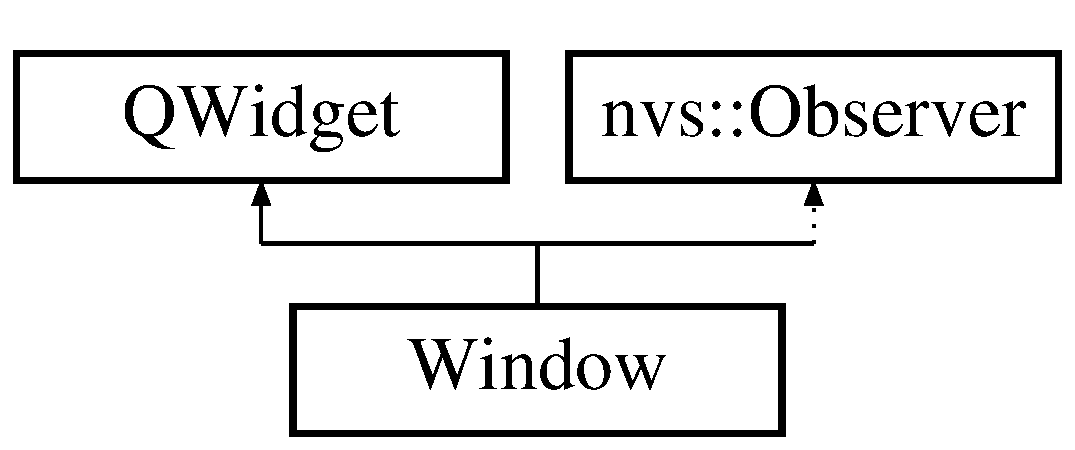
\includegraphics[height=2.000000cm]{class_window}
\end{center}
\end{figure}
\subsection*{Public Member Functions}
\begin{DoxyCompactItemize}
\item 
\mbox{\hyperlink{class_window_a2bbdf5c5bf31fa440a4f6a11e6916093}{Window}} (Labyrinth $\ast$game)
\begin{DoxyCompactList}\small\item\em constructeur du \mbox{\hyperlink{class_window}{Window}} \end{DoxyCompactList}\item 
Q\+Widget $\ast$ \mbox{\hyperlink{class_window_a1a60012c708f7e312c7c084ff923681c}{get\+Window}} ()
\begin{DoxyCompactList}\small\item\em get\+Window \end{DoxyCompactList}\item 
Q\+Spin\+Box $\ast$ \mbox{\hyperlink{class_window_acc5670401d2edec488b8eba20cfb1d2b}{get\+Y\+Position}} ()
\begin{DoxyCompactList}\small\item\em accede a la Position y \end{DoxyCompactList}\item 
Q\+Spin\+Box $\ast$ \mbox{\hyperlink{class_window_a4748fb7d7a0de845106effeec06a30a5}{get\+X\+Position}} ()
\begin{DoxyCompactList}\small\item\em accede a la Position x \end{DoxyCompactList}\item 
Q\+Spin\+Box $\ast$ \mbox{\hyperlink{class_window_ad4653c5a933dad023b65a13e41542f7b}{get\+X\+Case}} ()
\begin{DoxyCompactList}\small\item\em accede a la case x \end{DoxyCompactList}\item 
Q\+Spin\+Box $\ast$ \mbox{\hyperlink{class_window_a4ce8d19246d36b345acb0b25a4693572}{get\+Y\+Case}} ()
\begin{DoxyCompactList}\small\item\em accede a la case y \end{DoxyCompactList}\item 
Q\+Push\+Button $\ast$ \mbox{\hyperlink{class_window_a1ae19e5cb4129fcf241af162e00ccb99}{get\+Button\+Go}} ()
\begin{DoxyCompactList}\small\item\em accede au Button pour jouer \end{DoxyCompactList}\item 
Q\+Push\+Button $\ast$ \mbox{\hyperlink{class_window_ab97872ecccc1e1019ca123fb3643c864}{get\+Button\+Place}} ()
\begin{DoxyCompactList}\small\item\em accede au Button\+Place \end{DoxyCompactList}\item 
void \mbox{\hyperlink{class_window_affdeb2564502d9f4ca63e8c0c0c6f7c0}{update}} (const \mbox{\hyperlink{classnvs_1_1_subject}{nvs\+::\+Subject}} $\ast$subject) override
\begin{DoxyCompactList}\small\item\em mise a jour du jeu \end{DoxyCompactList}\item 
\mbox{\Hypertarget{class_window_a3706148bcb45e3989d378f2b58d58219}\label{class_window_a3706148bcb45e3989d378f2b58d58219}} 
void \mbox{\hyperlink{class_window_a3706148bcb45e3989d378f2b58d58219}{place\+Case}} ()
\begin{DoxyCompactList}\small\item\em placer une case ds le labyrinthe \end{DoxyCompactList}\item 
\mbox{\Hypertarget{class_window_a89ff44536707ce6fce5465b83add9dd4}\label{class_window_a89ff44536707ce6fce5465b83add9dd4}} 
void \mbox{\hyperlink{class_window_a89ff44536707ce6fce5465b83add9dd4}{go}} ()
\begin{DoxyCompactList}\small\item\em methode pour lancer le mouvement choisis \end{DoxyCompactList}\item 
\mbox{\Hypertarget{class_window_a455f9cf515c7bc78aa0c02b8530f777a}\label{class_window_a455f9cf515c7bc78aa0c02b8530f777a}} 
void \mbox{\hyperlink{class_window_a455f9cf515c7bc78aa0c02b8530f777a}{rotate\+Case}} ()
\begin{DoxyCompactList}\small\item\em rotate\+Case \end{DoxyCompactList}\end{DoxyCompactItemize}
\subsection*{Private Attributes}
\begin{DoxyCompactItemize}
\item 
\mbox{\Hypertarget{class_window_ac37243d4a26d082e4a255b0a07072227}\label{class_window_ac37243d4a26d082e4a255b0a07072227}} 
Q\+Spin\+Box $\ast$ {\bfseries x\+Case\+\_\+}
\item 
\mbox{\Hypertarget{class_window_a178347052c2e583403d9fb3a904806d1}\label{class_window_a178347052c2e583403d9fb3a904806d1}} 
Q\+Spin\+Box $\ast$ {\bfseries y\+Case\+\_\+}
\item 
\mbox{\Hypertarget{class_window_a0454f5b98fc9b1991ccb823ec1450985}\label{class_window_a0454f5b98fc9b1991ccb823ec1450985}} 
Q\+Spin\+Box $\ast$ {\bfseries x\+Position\+\_\+}
\item 
\mbox{\Hypertarget{class_window_a165c2b7c29c7f7f1f0f8df7c77a9063b}\label{class_window_a165c2b7c29c7f7f1f0f8df7c77a9063b}} 
Q\+Spin\+Box $\ast$ {\bfseries y\+Position\+\_\+}
\item 
\mbox{\Hypertarget{class_window_aa5aec3ff4cb51b5d23832a8991ab8679}\label{class_window_aa5aec3ff4cb51b5d23832a8991ab8679}} 
Q\+Push\+Button $\ast$ {\bfseries place\+\_\+}
\item 
\mbox{\Hypertarget{class_window_a419d02c3c1a37aff30fba1fc5c70e9f7}\label{class_window_a419d02c3c1a37aff30fba1fc5c70e9f7}} 
Q\+Push\+Button $\ast$ {\bfseries go\+\_\+}
\item 
\mbox{\Hypertarget{class_window_a29f73782c41d702337a59185d1279f57}\label{class_window_a29f73782c41d702337a59185d1279f57}} 
Q\+Push\+Button $\ast$ {\bfseries rotate\+Button\+\_\+}
\item 
\mbox{\Hypertarget{class_window_a1c64e9f2482f4e16bdf09398970ac804}\label{class_window_a1c64e9f2482f4e16bdf09398970ac804}} 
\mbox{\hyperlink{class_board}{Board}} $\ast$ {\bfseries board\+\_\+}
\item 
\mbox{\Hypertarget{class_window_a8fe8073d764a6c8ec30172e1acc6e965}\label{class_window_a8fe8073d764a6c8ec30172e1acc6e965}} 
Labyrinth $\ast$ {\bfseries game\+\_\+}
\item 
\mbox{\Hypertarget{class_window_acae5895788d29989c7de4dd86dfa5ff7}\label{class_window_acae5895788d29989c7de4dd86dfa5ff7}} 
Q\+Widget $\ast$ {\bfseries tagger\+Box\+\_\+}
\item 
\mbox{\Hypertarget{class_window_a5eb9980abfa1b99b171df6a9968bba98}\label{class_window_a5eb9980abfa1b99b171df6a9968bba98}} 
Q\+Label $\ast$ {\bfseries player\+Name\+\_\+}
\item 
\mbox{\Hypertarget{class_window_a27f2dc15c67d87d5cd112a7fb91dd19f}\label{class_window_a27f2dc15c67d87d5cd112a7fb91dd19f}} 
Q\+Label $\ast$ {\bfseries objective\+Blue\+\_\+}
\item 
\mbox{\Hypertarget{class_window_a225b362a376257c50161cea79b1377d8}\label{class_window_a225b362a376257c50161cea79b1377d8}} 
Q\+Label $\ast$ {\bfseries objective\+Green\+\_\+}
\item 
\mbox{\Hypertarget{class_window_a069de7a802d806df01e7c66038531fbb}\label{class_window_a069de7a802d806df01e7c66038531fbb}} 
Q\+Label $\ast$ {\bfseries objective\+Yellow\+\_\+}
\item 
\mbox{\Hypertarget{class_window_ad1b44cc43f04e39286422fc8c11fa844}\label{class_window_ad1b44cc43f04e39286422fc8c11fa844}} 
Q\+Label $\ast$ {\bfseries objective\+Red\+\_\+}
\item 
\mbox{\Hypertarget{class_window_a65a8e256e5a31121a5ee673434a44c1f}\label{class_window_a65a8e256e5a31121a5ee673434a44c1f}} 
\mbox{\hyperlink{class_box}{Box}} $\ast$ {\bfseries remain\+Box\+\_\+}
\item 
\mbox{\Hypertarget{class_window_a07a75399b6de45c21b06a42f1aada603}\label{class_window_a07a75399b6de45c21b06a42f1aada603}} 
Q\+Label $\ast$ {\bfseries current\+Player\+\_\+}
\end{DoxyCompactItemize}
\subsection*{Additional Inherited Members}


\subsection{Constructor \& Destructor Documentation}
\mbox{\Hypertarget{class_window_a2bbdf5c5bf31fa440a4f6a11e6916093}\label{class_window_a2bbdf5c5bf31fa440a4f6a11e6916093}} 
\index{Window@{Window}!Window@{Window}}
\index{Window@{Window}!Window@{Window}}
\subsubsection{\texorpdfstring{Window()}{Window()}}
{\footnotesize\ttfamily Window\+::\+Window (\begin{DoxyParamCaption}\item[{Labyrinth $\ast$}]{game }\end{DoxyParamCaption})}



constructeur du \mbox{\hyperlink{class_window}{Window}} 


\begin{DoxyParams}{Parameters}
{\em game} & \\
\hline
\end{DoxyParams}


\subsection{Member Function Documentation}
\mbox{\Hypertarget{class_window_a1ae19e5cb4129fcf241af162e00ccb99}\label{class_window_a1ae19e5cb4129fcf241af162e00ccb99}} 
\index{Window@{Window}!get\+Button\+Go@{get\+Button\+Go}}
\index{get\+Button\+Go@{get\+Button\+Go}!Window@{Window}}
\subsubsection{\texorpdfstring{get\+Button\+Go()}{getButtonGo()}}
{\footnotesize\ttfamily Q\+Push\+Button $\ast$ Window\+::get\+Button\+Go (\begin{DoxyParamCaption}{ }\end{DoxyParamCaption})\hspace{0.3cm}{\ttfamily [inline]}}



accede au Button pour jouer 

\begin{DoxyReturn}{Returns}

\end{DoxyReturn}
\mbox{\Hypertarget{class_window_ab97872ecccc1e1019ca123fb3643c864}\label{class_window_ab97872ecccc1e1019ca123fb3643c864}} 
\index{Window@{Window}!get\+Button\+Place@{get\+Button\+Place}}
\index{get\+Button\+Place@{get\+Button\+Place}!Window@{Window}}
\subsubsection{\texorpdfstring{get\+Button\+Place()}{getButtonPlace()}}
{\footnotesize\ttfamily Q\+Push\+Button $\ast$ Window\+::get\+Button\+Place (\begin{DoxyParamCaption}{ }\end{DoxyParamCaption})\hspace{0.3cm}{\ttfamily [inline]}}



accede au Button\+Place 

\begin{DoxyReturn}{Returns}

\end{DoxyReturn}
\mbox{\Hypertarget{class_window_a1a60012c708f7e312c7c084ff923681c}\label{class_window_a1a60012c708f7e312c7c084ff923681c}} 
\index{Window@{Window}!get\+Window@{get\+Window}}
\index{get\+Window@{get\+Window}!Window@{Window}}
\subsubsection{\texorpdfstring{get\+Window()}{getWindow()}}
{\footnotesize\ttfamily Q\+Widget$\ast$ Window\+::get\+Window (\begin{DoxyParamCaption}{ }\end{DoxyParamCaption})\hspace{0.3cm}{\ttfamily [inline]}}



get\+Window 

\begin{DoxyReturn}{Returns}

\end{DoxyReturn}
\mbox{\Hypertarget{class_window_ad4653c5a933dad023b65a13e41542f7b}\label{class_window_ad4653c5a933dad023b65a13e41542f7b}} 
\index{Window@{Window}!get\+X\+Case@{get\+X\+Case}}
\index{get\+X\+Case@{get\+X\+Case}!Window@{Window}}
\subsubsection{\texorpdfstring{get\+X\+Case()}{getXCase()}}
{\footnotesize\ttfamily Q\+Spin\+Box $\ast$ Window\+::get\+X\+Case (\begin{DoxyParamCaption}{ }\end{DoxyParamCaption})\hspace{0.3cm}{\ttfamily [inline]}}



accede a la case x 

\begin{DoxyReturn}{Returns}

\end{DoxyReturn}
\mbox{\Hypertarget{class_window_a4748fb7d7a0de845106effeec06a30a5}\label{class_window_a4748fb7d7a0de845106effeec06a30a5}} 
\index{Window@{Window}!get\+X\+Position@{get\+X\+Position}}
\index{get\+X\+Position@{get\+X\+Position}!Window@{Window}}
\subsubsection{\texorpdfstring{get\+X\+Position()}{getXPosition()}}
{\footnotesize\ttfamily Q\+Spin\+Box $\ast$ Window\+::get\+X\+Position (\begin{DoxyParamCaption}{ }\end{DoxyParamCaption})\hspace{0.3cm}{\ttfamily [inline]}}



accede a la Position x 

\begin{DoxyReturn}{Returns}

\end{DoxyReturn}
\mbox{\Hypertarget{class_window_a4ce8d19246d36b345acb0b25a4693572}\label{class_window_a4ce8d19246d36b345acb0b25a4693572}} 
\index{Window@{Window}!get\+Y\+Case@{get\+Y\+Case}}
\index{get\+Y\+Case@{get\+Y\+Case}!Window@{Window}}
\subsubsection{\texorpdfstring{get\+Y\+Case()}{getYCase()}}
{\footnotesize\ttfamily Q\+Spin\+Box $\ast$ Window\+::get\+Y\+Case (\begin{DoxyParamCaption}{ }\end{DoxyParamCaption})\hspace{0.3cm}{\ttfamily [inline]}}



accede a la case y 

\begin{DoxyReturn}{Returns}

\end{DoxyReturn}
\mbox{\Hypertarget{class_window_acc5670401d2edec488b8eba20cfb1d2b}\label{class_window_acc5670401d2edec488b8eba20cfb1d2b}} 
\index{Window@{Window}!get\+Y\+Position@{get\+Y\+Position}}
\index{get\+Y\+Position@{get\+Y\+Position}!Window@{Window}}
\subsubsection{\texorpdfstring{get\+Y\+Position()}{getYPosition()}}
{\footnotesize\ttfamily Q\+Spin\+Box $\ast$ Window\+::get\+Y\+Position (\begin{DoxyParamCaption}{ }\end{DoxyParamCaption})\hspace{0.3cm}{\ttfamily [inline]}}



accede a la Position y 

\begin{DoxyReturn}{Returns}

\end{DoxyReturn}
\mbox{\Hypertarget{class_window_affdeb2564502d9f4ca63e8c0c0c6f7c0}\label{class_window_affdeb2564502d9f4ca63e8c0c0c6f7c0}} 
\index{Window@{Window}!update@{update}}
\index{update@{update}!Window@{Window}}
\subsubsection{\texorpdfstring{update()}{update()}}
{\footnotesize\ttfamily void Window\+::update (\begin{DoxyParamCaption}\item[{const \mbox{\hyperlink{classnvs_1_1_subject}{nvs\+::\+Subject}} $\ast$}]{subject }\end{DoxyParamCaption})\hspace{0.3cm}{\ttfamily [override]}, {\ttfamily [virtual]}}



mise a jour du jeu 


\begin{DoxyParams}{Parameters}
{\em subject} & \\
\hline
\end{DoxyParams}


Implements \mbox{\hyperlink{classnvs_1_1_observer_a4c0373c644180bdc48558e5248968b3a}{nvs\+::\+Observer}}.



The documentation for this class was generated from the following files\+:\begin{DoxyCompactItemize}
\item 
C\+:/\+Users/benaz/\+Documents/cpp+/\+Labyrinth\+Project/window.\+h\item 
C\+:/\+Users/benaz/\+Documents/cpp+/\+Labyrinth\+Project/window.\+cpp\end{DoxyCompactItemize}

\chapter{File Documentation}
\hypertarget{observer_8h}{}\section{C\+:/\+Users/benaz/\+Documents/cpp+/\+Labyrinth\+Project/observer.h File Reference}
\label{observer_8h}\index{C\+:/\+Users/benaz/\+Documents/cpp+/\+Labyrinth\+Project/observer.\+h@{C\+:/\+Users/benaz/\+Documents/cpp+/\+Labyrinth\+Project/observer.\+h}}


Définition de la classe \mbox{\hyperlink{classnvs_1_1_observer}{nvs\+::\+Observer}}.  


\subsection*{Classes}
\begin{DoxyCompactItemize}
\item 
class \mbox{\hyperlink{classnvs_1_1_observer}{nvs\+::\+Observer}}
\begin{DoxyCompactList}\small\item\em Classe abstraite de base de tout observateur. \end{DoxyCompactList}\end{DoxyCompactItemize}
\subsection*{Namespaces}
\begin{DoxyCompactItemize}
\item 
 \mbox{\hyperlink{namespacenvs}{nvs}}
\begin{DoxyCompactList}\small\item\em Espace de nom de Nicolas Vansteenkiste. \end{DoxyCompactList}\end{DoxyCompactItemize}


\subsection{Detailed Description}
Définition de la classe \mbox{\hyperlink{classnvs_1_1_observer}{nvs\+::\+Observer}}. 


\hypertarget{subject_8cpp}{}\section{C\+:/\+Users/benaz/\+Documents/cpp+/\+Labyrinth\+Project/subject.cpp File Reference}
\label{subject_8cpp}\index{C\+:/\+Users/benaz/\+Documents/cpp+/\+Labyrinth\+Project/subject.\+cpp@{C\+:/\+Users/benaz/\+Documents/cpp+/\+Labyrinth\+Project/subject.\+cpp}}


Implémentation de la classe \mbox{\hyperlink{classnvs_1_1_subject}{nvs\+::\+Subject}}.  


{\ttfamily \#include \char`\"{}subject.\+h\char`\"{}}\newline
{\ttfamily \#include \char`\"{}observer.\+h\char`\"{}}\newline
\subsection*{Namespaces}
\begin{DoxyCompactItemize}
\item 
 \mbox{\hyperlink{namespacenvs}{nvs}}
\begin{DoxyCompactList}\small\item\em Espace de nom de Nicolas Vansteenkiste. \end{DoxyCompactList}\end{DoxyCompactItemize}


\subsection{Detailed Description}
Implémentation de la classe \mbox{\hyperlink{classnvs_1_1_subject}{nvs\+::\+Subject}}. 


\hypertarget{subject_8h}{}\section{C\+:/\+Users/benaz/\+Documents/cpp+/\+Labyrinth\+Project/subject.h File Reference}
\label{subject_8h}\index{C\+:/\+Users/benaz/\+Documents/cpp+/\+Labyrinth\+Project/subject.\+h@{C\+:/\+Users/benaz/\+Documents/cpp+/\+Labyrinth\+Project/subject.\+h}}


Définition de la classe \mbox{\hyperlink{classnvs_1_1_subject}{nvs\+::\+Subject}}.  


{\ttfamily \#include $<$set$>$}\newline
\subsection*{Classes}
\begin{DoxyCompactItemize}
\item 
class \mbox{\hyperlink{classnvs_1_1_subject}{nvs\+::\+Subject}}
\begin{DoxyCompactList}\small\item\em Classe de base de tout \char`\"{}sujet d\textquotesingle{}observation\char`\"{}. \end{DoxyCompactList}\end{DoxyCompactItemize}
\subsection*{Namespaces}
\begin{DoxyCompactItemize}
\item 
 \mbox{\hyperlink{namespacenvs}{nvs}}
\begin{DoxyCompactList}\small\item\em Espace de nom de Nicolas Vansteenkiste. \end{DoxyCompactList}\end{DoxyCompactItemize}


\subsection{Detailed Description}
Définition de la classe \mbox{\hyperlink{classnvs_1_1_subject}{nvs\+::\+Subject}}. 


%--- End generated contents ---

% Index
\backmatter
\newpage
\phantomsection
\clearemptydoublepage
\addcontentsline{toc}{chapter}{Index}
\printindex

\end{document}
